\documentclass{sig-alternate}
\usepackage{mdwlist}
\usepackage{url}
\usepackage{graphicx}

\begin{document} 

\title{MelTS}
\subtitle{Melody Translation System}
\numberofauthors{2}
\author{
\alignauthor Nicole Limtiaco \\ \email{limni@seas.upenn.edu} \\ Univ. of Pennsylvania \\ Philadelphia, PA
\alignauthor Rigel Swavely \\ \email{rigel@seas.upenn.edu} \\ Univ. of Pennsylvania \\ Philadelphia, PA}
\date{}
\maketitle

\begin{abstract}
  \textit{MelTS is an automatic harmonization system that creates multi-part arrangements
  in the style of the data on which it was trained. The system approaches the problem
  of harmonization from a machine tranlsation perspective, modeling the melody of a song
  as the source language and each harmony as a target language. The approach stands in
  contrast to previous approaches to the harmonization problem, which have primarily 
  taken two forms: satisfying rules provided by music theory or predicting
  the chord under the melody. A major benefit of the MelTS approach is that
  the style of the harmony voices can be learned directly from the training data, 
  just as vocabulary and structure can be learned from a parallel  corpus of natural languages. In particular, generating harmony lines probabilistically and individually, as opposed to by rule satisfaction or as a consequence of a predicted chord, allows for the production of more natural arrangements without the need for simplifying assumptions about the structure of the music to be produced.}
\end{abstract}

\section{Introduction}
\label{sec:intro}
Multi-part musical arrangements are a cornerstone of many musical styles. From choirs and string quartets to barbershop and a-cappella groups, musicians are constantly producing creative arrangements to harmonize with their favorite melodies. The automatic harmonization problem is one in which machines are put to this uniquely human task of composing music to support a melody. 

Formally, a \textit{melody} is a sequence of input \textit{notes}, where each note contains information
about pitch and timing. A \textit{harmony} is a sequence of output notes which are produced with
the constraint that the sequence of notes supports the input melody. Both \textit{melodies} and \textit{harmonies} may be referred to as \textit{parts} in an arrangement. The term \textit{voice}
is defined as some category of \textit{parts} with a certain set of identifying 
characteristics. For example, the bass lines in rock music are one type of voice and the soprano solos in an 
opera are another. The aim of the automatic harmonization problem is to, given a melody part, generate parts in $n$ different harmony voices that, when played together, sound coherent and pleasant.

MelTS, a melody translation system, is a proof of concept endeavor aimed at reducing the automatic harmonization problem to a machine translation problem, viewing the melody voice as the source language and the harmony voices as the targets. Such an approach allows the style of the desired harmonies to be learned from a set of musical training data, just as the intricacies of a natural language can be learned from a parallel corporus.

\section{Related Work}
\label{sec:related_work}
\subsection{Automatic Harmonization}
Automatic harmonization is a subset of the automatic musical composition problem,
which dates as far back as the field of artificial intelligence itself. Perhaps
the earliest work in automatic composition is Hiller and Isaacson's
\textit{Illiac Suite} \cite{hiller1959experimental}, which is widely accepted as being the first
musical piece composed by an electronic computer. Hiller and Isaacson
used a generate-and-test method that generated musical phrases psuedo-randomly and 
kept only those that adhered to a set of music-theory-inspired heuristics. 

Staying in line with the use of musical rules, Ebcio\v{g}lu \cite{Ebci̇oğlu1990145} provided a break-through 
in the specific field of automatic harmonization through his CHORAL system. CHORAL, 
bolstered by about 350 music-theory and style rules expressed in first order logic, performed the task of
writing four-part harmonies in the style of J.S. Bach. With these logical predicates, Ebcio\v{g}lu 
reduced the problem of composing a harmony to a simple constraint satisfaction problem. Similar 
later works, notably by Tsang \& Aitkin \cite{tsang1991}, also crafted the harmonization problem as a 
problem in constraint satisfaction, but with a significantly smaller amount ($\sim$20) of musical rules.
The result of these constraint-based works were musically sensible; however,
crafting the constraints such that the output is musical requires deep, human knowledge about music in general and about the style of music to be produced in particular.

More recent works have put data-driven methods into use in order to infer the patterns that govern real compositions. A simple case-based model implemented by Sabater \textit{et al.} \cite{Sabater98usingrules} was built to generate
accompanying chords for a melody line. To a choose a harmony chord for a given context of previous
harmony chords and the currently sounding melody note, the system would check a case base to see if any
cases had the same harmony context and melody note and use the corresponding harmony chord if such a 
match were found. Musical heuristics were used to generate a chord if no match was found in the case base.
An automatic harmonizer utilizing neural networks was also built by Hild \textit{et al.} \cite{NIPS1991_576}  to produce a harmony
chord for a given melody quarter beat. Input features to the network included harmony context, current melody pitch,
and whether or not the beat was stressed.

As these examples show, the previous harmony context and the melody pitch are important signals in deciding
what the current harmony phrase should be. Many works have been conducted that model these signals using
n-gram Markov Models. A Markov model assigns probabilities to some event $C_{t}$ conditioned on a limited history
of previous events [$C_{t-1}\ldots\\
C_{t-n}$], implictly making the assumption that the event $C_{t}$ depends only on a 
small amount of information about its context. For example, a system called MySong produced by Simon \textit{et al.} \cite{export:64277}
generates chord accompaniment given a vocalized melody by using a 2-gram Markov model for the harmony
context and a 2-gram Markov model for the melody context. A similar system implented by Scholz \textit{et al.} \cite{4959518},
which also generates chord accompanimants, experimented with 3-gram to 5-gram Markov models and incorporated
smoothing techniques commonly seen in NLP to account for cases in which the model has not seen a context
that is present in the test data. Most recently, Raczy\'{n}ski \textit{et al.} \cite{doi:10.1080/09298215.2013.822000} uses discriminative Markov models that
model harmony context, melody context, and additionaly the harmony relationship to the tonality.

A recent senior design project out of the University of Pennsylvania by Cerny \textit{et al.} \cite{UAMP} also used melody pitch and previous harmony context
as their main signals for determining the next harmony chord to generate. However, they used these
signals as inputs to an SVM classifier, as opposed to training a Markov model. 

\subsection{Machine Translation}
MelTS reduces the automatic harmonization problem to a machine translation problem. However, automatic harmonization differs in an interesting way from standard machine translation applications in that it requires translation from one language (melody voice) to many languages ($n$ harmony voices) instead of one language to one other language. Looked at from a different perspective, the problem can be seen as a sequence of translations from many source languages to one target language. The sources are the melody voice and all the harmony voices, if any, that have been produced so far; the target is the harmony voice to be produced next. Though limited work has been done on the multi-source translation problem, Och and Ney \cite{franzjosefochhermannney2001} produced a work describing several ways of altering standard methods to deal with multiple sources.

\section{System Model}
\label{sec:sys_model}
\subsection{Motivating the Machine Translation Approach}

The previous data driven approaches applied to automatic harmonization all share in the fact that they predict the chords to be played under the input melody. Automatic harmonization via chord prediction imposes two major limitiations: a limited set of producible chords and a lack of fluid movement within the individual parts. 

In the best case, chord prediction will alow only the generation of those chords seen in the training data. In more restrictive set-ups where classification algorithms are used, the chord predicted is based on a classifier choosing from a relatively small number of chord classes. Some chord prediction systems do not generate individual parts at all, but rather view the harmony output as just the underlying chord sequence generated. If individual parts are produced, the notes for each part are chosen from the predicted chord, not based on the context of previous notes in that part. Chord prediction further limits interesting musical structure since some assumptions must be made about when the predicted chord is to be played. This is a far cry from actual musical arrangements, whose parts can move independently of each other and at times produce non-conventional chords. In fact, this approach differs greatly from how actual composers create multi-part arrangements, creating musical phrases in each part rather than purely choosing chords to sound on each beat.

Predicting the note sequences for individual parts in such a way that will allow them to sound consonant when played together can bypass many of the pitfalls of chord prediction. 
Such an approach will allow unseen chords to be produced because there is no restriction on which groups of notes can sound simultaneously, only on which notes can be produced. Furthermore, the system can be made to encourage interesting movement within the individual parts, for example by taking the part's context into account and by allowing rhythmic variation. Machine translation techniques are used to achieve these goals of simultaneous consonance and part fluidity.

There are two main analogies between natural languages and musical voices that motivate the usage of machine translation techniques for automatic harmonization. The first analogy is that both natural languages and musical voices have a sense of ``word translations''. Just as there may be several words in the target language that could be sensible translations of a given word in the source 
langauge, there are also several notes in the harmony voice that can harmonize well with an input melody note. Importantly, however, it is not the case that any note can harmonize well with the melody note. Some notes will sound dissonant when played together and still other notes may not be in the harmony voice at all, since harmony voices may have specific note ranges. The second analogy is that both natural languages and musical voices have a concept of ``fluency'', the idea that only certain strings of tokens (i.e. words or notes) are sensible. For example, the statement ``is name my John'' contains all English words but is unlikely to be understood by an English speaker since that string of words is meaningless based on the syntactic rules of the language. Similarly, a random sequence of notes may not sound sensible in the context of its harmony voice, if the notes are recognized as music at all. Since machine translation techniques can produce novel natural language utterances based on the properties of word translations and fluency, it follows that novel musical parts can be generated with the same techniques.

\subsection{System Design Overview}

In line with the analogies explained above, two probabilistic models commonly seen in statistical machine translation are employed: the language model and the translation model. The language model, denoted as $L(H)$, provides a probability for a sequence of pitches in a harmony part. The translation model is made up of two sub-models: the note model, denoted $N(M|H)$, and the phrase model, denoted $Ph(M|H)$. The note model provides a probability of harmonization between melody and harmony pitches. The phrase model provides a probability of harmonization between two-note musical phrases, consisting of pitch and rhythm information, between the meldoy and the harmony. Specifically, the models are given by the formulas below: 
\\

$L(H) = \Pi_{i = 1}^{l} P[pitch(h_{i}) | pitch(h_{i - 1}) \ldots pitch(h_{i - n})]$\\

$N(M | H) = \Pi_{i = 1}^{l} P[pitch(m_{i}) | pitch(h_{j})]$\\

$Ph(M | H) = \Pi_{i = 1}^{l - 1} P[(m_{i}, m_{i + 1}) | (h_{j} \ldots h_{j + k})]$\\
\\

The model scores for a generated harmony are combined into a total score using a weighted log-linear model. In general, a log-linear model computes a sum of the features' values each multiplied by its corresponding weight. The model adapted to this application is defined below:\\

$S(H | M) = [w_{L}\cdot log(L(H))] + $\\

$[w_{Ph}\cdot log(Ph(M | H))] + [w_{N}\cdot log(N(M | H))]$\\

A learning algorithm is used to determine the values of $L(H)$, $N(M | H)$, and $Ph(M | H)$ based on a set of music training data. The weights corresponding to the models are determined with a weight-optimization algorithm that optimizes over a separate set of music data. The details of the alrogithms are discussed in the implementation section.

Given a melody part $M$, the goal is to find some harmony part $H$ that maximizes the score $S(H | M)$.
A decoder utilizing  the language and tranlsation models is employed to find the harmony part in the search space that maximizes the weighted log-linear score for the given melody part. Figure 1 shows a graphical overview of the model just described.
\begin{figure}
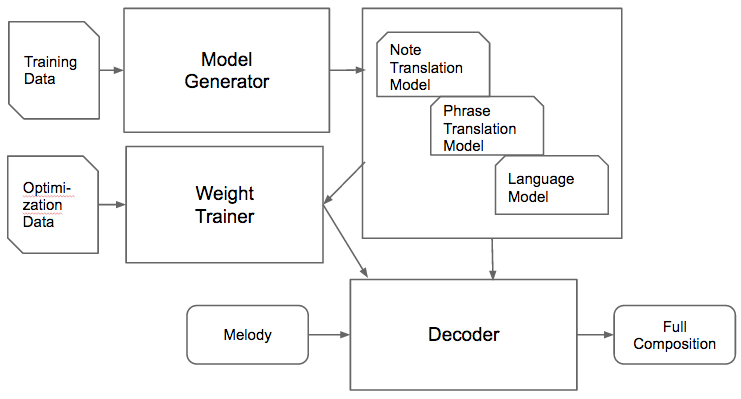
\includegraphics[scale=0.3]{system_design.png}
\caption{Overview of System Design}
\end{figure}

Up until this point, it has been assumed that the translation is into only one harmony voice. However, the goal is to produce a complete $n$-part arrangement. In order to do this, the decoding portion of the system is viewed as a sequence of multi-source translations where the source languages are the melody voice and all of the harmony voices generated so far. The generated harmony maximizes a weighted log-linear score that incorporates its language model score and the scores given by each translation model from one of the existing voices to it. Specifically, given a set $V$ of source voices, the multi-source version of problem finds a harmony part $H$ such that\\

$H = \underset{H}{argmax}\ S(H | V) = [w_{L}\cdot log(L(H))] + $\\

$[w_{N}\cdot \Sigma_{v \in V} log(N(v | H))] + [w_{Ph}\cdot \Sigma_{v \in V} log(Ph(v | H))]$\\

Viewing translation as a sequence of generation steps then introduces the problem of determining the best order for the parts to be generated. Since each part is constrained by the parts generated previously, one would expect that the order in which the parts are generated will have an observable affect on the output. Indeed,  experiments have shown that the quality of the output varies greatly among different generation orderings. Details about how an optimal ordering is choosen will be discussed in the implementation section.

\section{System Implementation}
\label{sec:sys_implement}
\subsection{Data Collection and Interaction}
To interact with music data, a third-party software called Music21\cite{Cuthbert_music21:a} was used. Music21 is a library developed at MIT which provides a simple API for querying several types of music formats.  MusicXML, a type of encoding for standard music notation, is the primary data format used. This format can be parsed by Music21 into Stream objects which can then be queried for any of the information contained in the notation, including key, tempo, and notes with pitch and timing. 
\subsubsection{Bach Data}
The Music21 package has a library of over $2,000$ compositions, mostly written by classical composers. The package's extensive collection of Bach chorales --- which each have soprano, alto, tenor, and bass voices --- was used as the main source of training, optimization, and test data. Table 1 gives information regarding the size of the Bach corpus.
\subsubsection{Barbershop Data}
In order to make sure the system was extensible and not optimized to just Bach chorales, a data set of barbershop music was also collected. Barbershop as a genre was chosen due to its musical difference with Bach chorales, generally including much more dissonance and less predictable harmonies. However, it is structurally similar to Bach in that it traditionally is written with four separate voices, making it easy to apply the system to both types of music. This data was gathered from various sources, largely in PDF format. These documents were parsed by Optical Music Recognition systems in order to convert them to MusicXML, so that they could be manipulated by the Music21 library. However, the scanning was far from perfect, and many of the scores required significant manual editing in order to be usable for the system. As such, many of the scores were simply discarded, and so the barbershop data was not large enough to perform the same robust evaluation as the Bach data set. However, it was large enough to train some models and produce very simple barbershop harmonies, which acted as a sanity check as changes were made to the system.

\begin{table}
  \begin{center}
      \begin{tabular}{| l | r | r | r | r | r |}
      \hline
       \  & Songs & S. Notes & A. Notes & T. Notes & B. Notes \\ \hline
       Total &  351 & 21062 & 25255 & 25691 & 25867 \\ 
       Major &  185 & 11371 & 13518 & 13647 & 13846 \\ 
       Minor & 166 & 9691 & 11737 & 12044 & 12021  \\ \hline
      \end{tabular}
  \end{center}
  \caption{Number of songs and notes in the training data set. ``S'' stands for soprano, ``A'' for alto, ``T'' for tenor, and ``B'' for bass}
\end{table}

\subsection{Note Representation}
Notes are represented in the models as strings of the form:\\
\\
\texttt{pitch -> \{pitch class\}\{octave\}}\\
\texttt{note -> \{pitch\}(,\{pitch\})*(:\{quarter-length duration\})?}\\
\\
Every model uses at least the pitch information for a note, so the pitch class and octave are necessary in the representation. For exmaple, the pitch representation of a middle C is \texttt{C4}. A chord, a group of notes that sound together in the same part, can be represented by repeating the pitch and octave portion of the representation. For example, a representation of a C-major chord would be \texttt{C4,E4,G4}. Since the phrase model incorporates timing information, the note representations in that model include the note's quarter-lengths appended to the pitches after a colon. For example, a middle C eighth note is represented as \texttt{C4:0.5}.

Rests, moments of silence in the composition, are considered as ``notes'' in the model. They are represented by the string \texttt{R}. Including rests makes it possible to harmonize a melody note with silence, thus offering some opportunity for rhythmic variation. However, including rests does pose the potential problem of producing too much silence, something which is generally not optimal for music generation. For example, imagine a language model of n-gram size $2$ in which $P(\texttt{R} | \texttt{R})$ and $P (\texttt{R} | \texttt{R}\ \texttt{R})$ are both relatively high. Once one rest is produced, the system may very well produce rests for the remainder of the song. Therefore, for fear of continually producing rests, all contiguous sequences of rests in the training data are treated as one rest \texttt{R} in the model.

Measure bars are also modeled as ``notes'' in the system. They are represented by the string \texttt{BAR}. A special measure bar, the bar at the end of last measure in the song, is given a special representation: \texttt{END}. These notes are slightly different in that they are only present in the language model. \texttt{BAR} and \texttt{END} can only be harmonized with actual measure bars and song end in the given melody part, so there is no need to include them in the translation model. The motivation for including \texttt{BAR} and \texttt{END} in the language model is that they provide information about where in the composition the system is trying to produce notes. This information is helpful because some notes may be more likely to start or end measures and some sequences of notes may be more likely to end a song. Coming back to the analogies between languages and musical voices, the \texttt{BAR} and \texttt{END} symbols can be likened to punctuation marks, which can give very strong cues about which words to generate.

\subsection{Model Generation}
The models represent probabilities of events as nested dictionaries. The outer dictionary maps the given event, $A$, to the inner dictionary, which maps the unknown event, $B$, to the probability $P(B | A)$. In the case of the language model, $A$ is the sequence of $(i - 1) ... (i - n)$ harmony pitches and $B$ is the $i^{th}$ harmony pitch, whereas in the note translation model, $A$ and $B$  are pitches in the harmony and melody, respectively, that sound simultaneously. Similarly in the phrase translation model, $A$ and $B$ are two-note sequences in the harmony and melody, respectively, that sound simultaneously.

The probabilities are calculated based on the counts of the events in the training compositions, plus smoothing techniques applied so that no event is assigned a zero probability. For now, the smoothing techniques are ommitted for ease of explanation. Formally, the language ngram probabilities are given by: \\

$P(pitch(h_{i}) | pitch(h_{i - 1}) ... pitch(h_{i - n})) = $\\

$\frac{count(pitch(h_{i}) \wedge pitch(h_{i - 1}) \wedge ... \wedge pitch(h_{i - n}))}{count(pitch(h_{i - 1}) \wedge ... \wedge pitch(h_{i - n}))}$\\

The note translation probabilities are given by:\\

$P(pitch(m_{i}) | pitch(h_{j})) = \frac{count(pitch(m_{i}) \wedge pitch(h_{j}))}{count(pitch(h_{j}))}$\\

and the phrase translation probabilities are given by:\\

$P((m_{i}, m_{i+1}) | (h_{j} \ldots h_{j+k})) = \frac{count((m_{i} \wedge m_{i+1}) \wedge (h_{j} \wedge \ldots \wedge h_{j+k}))}{count((h_{j} \wedge \ldots \wedge h_{j+k}))}$\\

The event $pitch(h_{i}) \wedge ... \wedge pitch(h_{i - n})$, as seen in the ngram probability formula, occurs whenever the pitches of notes $h_{i - n}, h_{i - n + 1}, ..., h_{i}$ appear contiguously in that order in the haromny part. 

The event $pitch(m_{i}) \wedge pitch(h_{j})$, as seen in the note translation probability formula, occurs whenever the pitch of note $m_{i}$ is sounding in the melody at the same time that the pitch of note $h_{j}$ is sounding in the harmony, regardless of when either note begins or ends. To compute these counts, the algorithm iterates through each note $m_{i}$ in the melody and update the counts for event $m_{i} \wedge h_{j}$ for all notes $h_{j}$ that have any portion of their duration sounding at the same time as any portion of the duration of $m_{i}$.

The counts for the events $(m_{i} \wedge m_{i+1}) \wedge (h_{j} \wedge \ldots \wedge h_{j+k})$, as seen in the phrase translation model probability formula, are gathered by moving a 2-note wide sliding window across the melody part
and determing, for each 2-note melody phrase, the phrase of notes $(h_{j} \ldots h_{j + k})$ that are playing simultaneously in the harmony part. Since the phrase translation model takes timing information into account, the training algorithm insures that the melody and harmony phrases have the same duration. If the first note in the harmony phrase begins sounding before the first note in the melody phrase, its duration in the model is shortened so that it only sounds when the first melody phrase note sounds. Similarly, if the last note in the harmony phrase finishes after the last note in the melody phrase, its duration in the model is shortened so that if finishes at the same time as last note in the melody phrase. For example, take the melody phrase \texttt{[C4:1.0 E4:1.0]} and the harmony phrase \texttt{[E4:1.0 C4:0.5 C4:0.25 G4:1.0]} which starts 0.5 of a quarter-length before the melody phrase. The corresponding harmony phrase event will be \texttt{[E4:0.5 C4:0.5 C4:0.25 G4:0.75]}. See Figure 1 for a pictoral explanation of phrase alignment.

\begin{figure}
	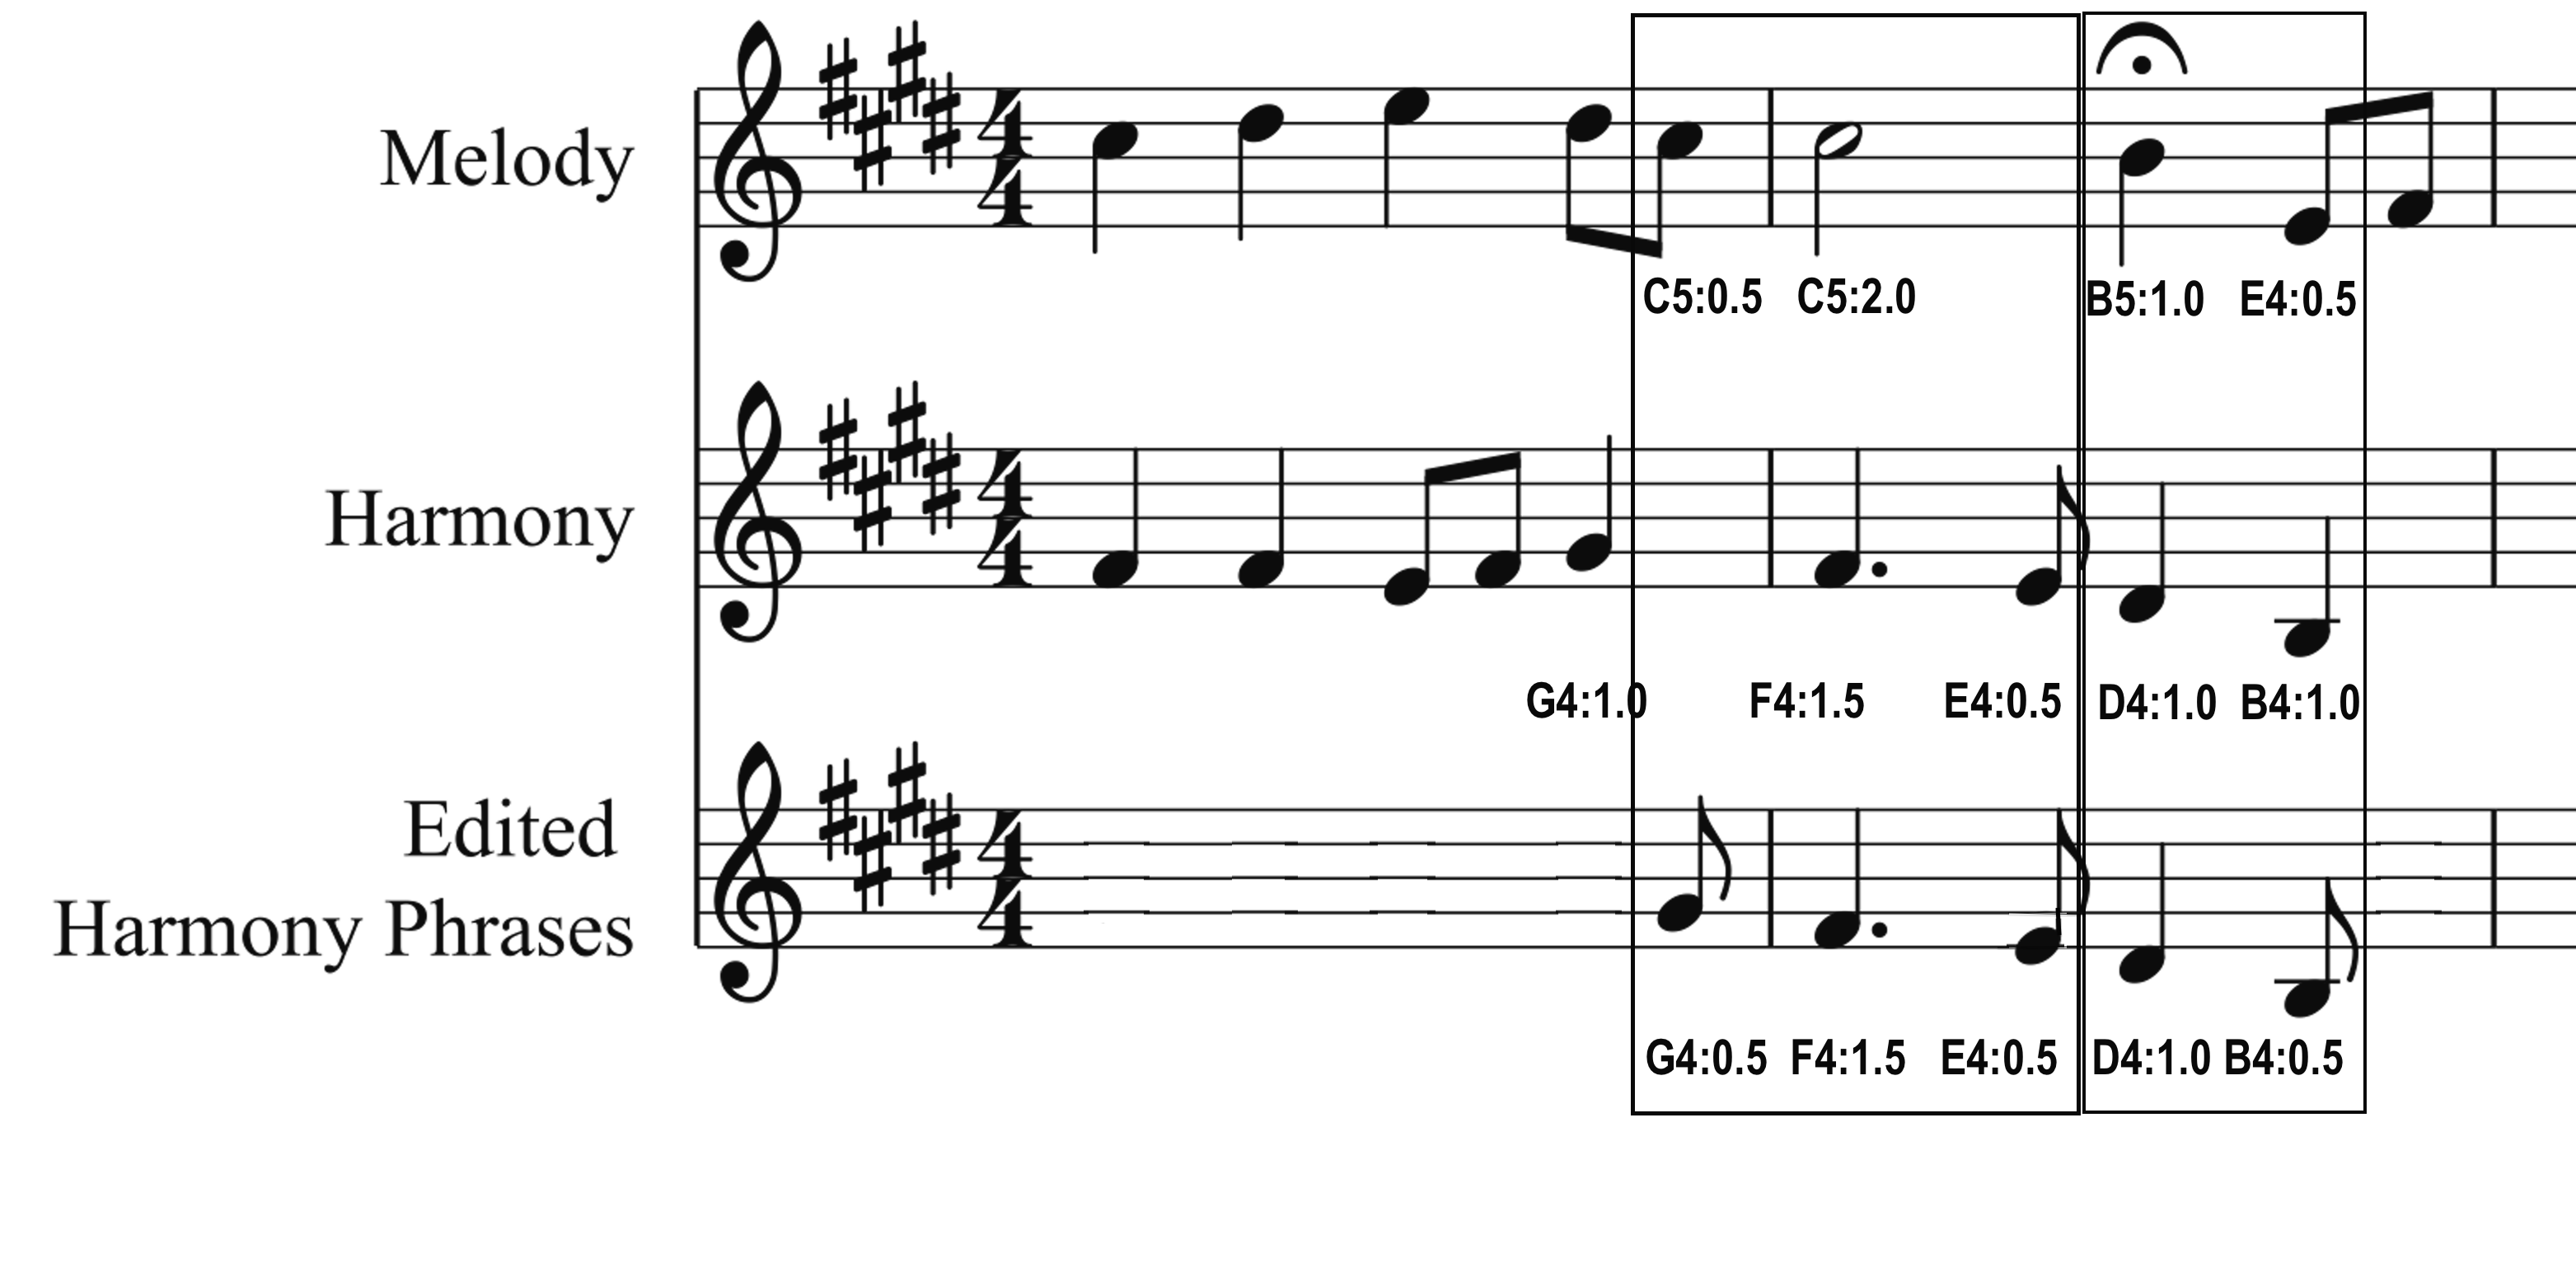
\includegraphics[scale=0.08]{./phrase_examples.png}
	\caption{Two phrase events are boxed. The original harmony part is displayed along with edited notes that line up with their corresponding melody phrase.}
\end{figure} 

Laplace smoothing, also known as additive smoothing, is incorporated into the language model to avoid any events having zero probability. Specifically, for some smoothing constant $\alpha$, the language ngram probabilities are given by: \\

$P(pitch(h_{i}) | pitch(h_{i - 1}) ... pitch(h_{i - n})) = $\\

$\frac{count(pitch(h_{i}) \wedge pitch(h_{i - 1}) \wedge ... \wedge pitch(h_{i - n})) + \alpha}{count(pitch(h_{i - 1}) \wedge ... \wedge pitch(h_{i - n})) + (48\alpha)}$\\

The constant $48$ in the equation above is meant to be the number of possible note values for the variable $h_{i}$. It is derived from the fact that there are 12 notes in each octave and that 4 is a very liberal estimate for how many octaves a particular voice can span. 

The translation models use a simple smoothing constant, $\alpha = 1e-10$, for when there is no probability associated with a translation event.

Lastly, the ngram size $n$ and smoothing parameter $\alpha$ have been choosen as $n = 3$ and $\alpha = 1e-10$. Qualitatively, it seems that these values are sufficient, though one could imagine optimizing these parameters to maximize the quality of the system output.

\subsection{Weight Trainer}
The weights for each model are tuned using the Powell algorithm \cite{Koehn:2010:SMT:1734086} on a set of held out music data, which overlaps with the test set but is separate from the data used to train the models. If the harmonies to be generated are for major songs, only the major compositions in the training data are used, and vice versa for minor songs. The algorithm tunes the weights to optimize an arbitrary metric; in this case, the weighted log-linear score was optimized. See Table 2 for information on the held out optimization set. 

\begin{table}[h]
  \begin{center}
      \begin{tabular}{| l | r | r | r | r | r |}
      \hline
       \  & Songs & S. Notes & A. Notes & T. Notes & B. Notes \\ \hline
       Total &  20 & 1178 & 1392 & 1413 & 1468 \\ 
       Major &  11 & 658 & 779 & 793 & 822 \\ 
       Minor & 9 & 520 & 613 & 620 & 646  \\ \hline
      \end{tabular}
  \end{center}
  \caption{Number of songs and notes in the held out training data set used for weight tuning. ``S'' stands for soprano, ``A'' for alto, ``T'' for tenor, and ``B'' for bass}
\end{table}

\subsection {Decoder}
The goal of the decoder is to find the harmony part $H$ such that $H$ maximizes the weighted log-linear score $S(H | M)$. However, the search space is much too large to enumerate all possible harmony parts in order to determine the best. Assuming the harmony voice spans no more than 4 octaves and that there are 12 notes in an octave, an exhaustive search of all harmony parts for a song with $n$ melody notes would require the inspection of $(12\cdot 4)^{n} = 48^{n}$ harmony parts. For an average length song comprised of $100$ melody notes, the number of possible harmony parts comes out to $48^{100} \approx 1.3\times10^{168}$. 

To shrink the search space, harmony parts are generated four measures at a time. That is, for each four measure chunk, a set of $k$ harmonies are generated. The cross-product of those $k$ harmonies with the stored harmonies corresponding to the previous measures result in a new set of full-song harmony prefixes, out of which the top ranking $j$ are stored for the next iteration.

The harmony generation process for a four-measure chunk is accomplished with a beam-seach decoder. Specifically, at every iteration $t$, the decoder will have a set of hypotheses $S_{t}$ where each hypothesis is a sequence of notes with a duration equivalent to the duration of the melody part up to its $min(2t, l)^{th}$ note, where $l$ is the total number of notes in the melody. The decoder is begun with the set $S_{0}$ containing only the empty hypothesis. 

For each two-note phrase in the melody, the decoder finds all possible harmony phrases that can sound with that melody phrase, call it $m_{i} = (m_{i}^{0}, m_{i}^{1})$. A portion of the harmony phrase possibilites comes from the corresponding harmony phrases for $m_{i}$ in the phrase translation model. The other possibilities are two-note phrases which have the same rhythm as $m_{i}$, but whose pitches are determined by the note translation model. The cross product of the pitches corresponding to $m_{i}^{0}$ with the pitches corresponding to $m_{i}^{1}$ in the note translation model give the pitches for this portion of the possible harmony phrases. There are two important things to note about generating possible harmonies from the phrase translation model. The first is that since the harmony and melody phrase pairs in the phrase translation model are always of the same duration, the harmony phrases can be added to the hypotheses without having to worry about duration mismatches between the hypotheses and the translated melody prefix. Secondly, the possible harmonies generated from the phrase translation model are the main source of rhythmic variation in the harmony generation algorithm. Those phrases are what prevents the output harmonies from being exactly lined up with the melody, leading to more natural-sounding arrangements.

Once the possible harmony phrases are retrieved, the decoder constructs $S_{t + 1}$ by examining each hypothesis in $S_{t}$. For each hypothesis $hyp \in S_{t}$, a new hypothesis is constructed for each possible harmony phrase $h$, where the new hypothesis is just $h$ appended to $hyp$. All the new hypotheses generated in this iteration are added to $S_{t + 1}$. After all the new hypotheses have been added, the hypotheses in $S_{t + 1}$ are sorted in descending order by their $S(hyp | m_{1} ... m_{min(2(t +1), l)})$ values, and only the top $k$ are saved for the next iteration.

\subsection {Generating Multiple Parts}
The decoder was decribed above with the assumption that there is only one melody voice for  which to create translations. In reality, when generating multiple harmony parts, the $j^{th}$ harmony voice generated will be constrained by several source voices: the melody voice, $M$ and the $j-1$ previous harmony voices generated. Let this set of source voices be defined as follows\\

$S^{j} = {M} \cup \{\ H^k | 1 \leq k \leq j- 1\ \} $\\

In order to grow a harmony hypothesis in this setup, the melody phrase occurring after the end of the hypothesis to be grown must be determined for each source voice. From there, the harmony phrase possibilities can be retrieved and appended to the hypothesis as described above. Note that the 2-note phrases from the souce voices may be of varying durations, resulting in the hypotheses being of varying durations. As a consequence of this, it is possible that the end of a harmony hypothesis may not line up with the end of a note in one of the source voices. Therefore, the 2-note phrases that are translated may actually be versions of the notes in the source voices whose beginning note durations are altered so that the phrase begins only when the hypothesis ends. For example, if a hypothesis has duration 2.0 and, for some $s \in S^{j}$, the phrase that begins at or before 2.0 quarter-lengths, denote it $(m_{i}, m_{i + 1})$, begins at 1.5 quarter-lengths, then the melody phrase to be translated from $s$ will be $(m_{i}, m_{i + 1})$, but $(m_{i})$ will have 0.5 quarter-lengths less of duration. 

As mentioned earlier, the order in which the parts are generated is important since each part is contrained on all the parts generated before it. One ordering option is to choose some arbitrary ordering that is believed to be sufficient. However, there is no guarantee that an ordering that produces nice sounding harmonies for several compositions will produce optimal harmonies for all compositions. Instead of arbitrary choice, a greedy search for the best ordering is used to generate the parts.

In the greedy search, all harmony voices not yet generated are generated with the current source voices. The voice with the highest weighted log-linear score is added to the source voices, and the process continues until all harmony voices to be generated are in the set of source voices. The intuition behind this method is that one would like to build up the musical arrangement with the strongest harmony voices possible.
It stands to reason that constraining the next harmony voice with high-quality source voices will lead to a higher quality generation than one which is constrained on low-quality source voices.

\section{System Performance}
\label{sec:sys_perform}
\subsection{Perplexity}
In order to evaluate the quality of the trained models, the perplexity metric, a common metric in natural language processing, is employed. This metric captures how well the algorithm scores arrangements in the test set. Perplexity $PP$ \cite{Koehn:2010:SMT:1734086} is defined over all compositions $c$ in a test set as:\\

$log_2 PP = - \sum_{c} log_2 S(H_{c} | M_{c})$\\

This measure provides a real number metric to evaluate different iterations of the system. Evaluations were done over 2 main test sets. One was a set of 27 major Bach chorales, pulled from the same corpus but not overlapping with the training data. The second was a set of 27 randomly generated compositions for the melodies of the same 27 Bach chorales, referred to as anti-examples. The purpose of training on these two sets was to give evaluation scores similar to precision and recall. A high perplexity on the anti-examples test set implies good precision, whereas a low perplexity on the Bach test set implies good recall. 	

This metric is used to compare a set of system iterations, including a system in which just the the note translation model and language model are used with equal weights, another system in which all three models are used but are weighted equally, and lastly the final system with weights tuned by the weight trainer. All three systems were trained on the same 185 major Bach chorales. Tables 3 and 4 show the perplexity results over the Bach and anti-example test sets, respectively. 

As shown in Table 3, each of the successive iterations of MelTS received better perplexity scores. The largest jump occured between the system with tuned weights versus the system without tuned weights, where most part combinations saw a jump of about a factor of a little over 4. In Table 3 and Table 4, it can also be seen that the perplexity of the anti-examples is consistently worse than the perplexity over the Bach chorales, although not by a significant amount until the final iteration. As seen in Figure 3 for the Soprano-Alto perplexity, the perplexity drops much faster for the gold standard Bach chorales than it does for the random harmonizations as a result of the last iteration.  

\begin{figure}
  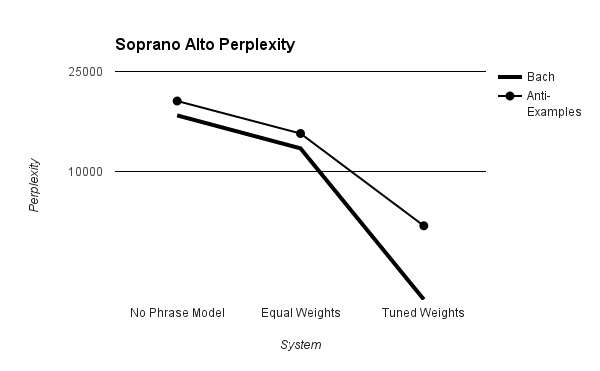
\includegraphics[scale=0.5]{soprano_alto_perplexity}
  \caption{Soprano Alto perplexity on all iterations of MelTS on a log scale.}
\end{figure}


\begin{table*}[t]
      \begin{tabular}{| l | l | l | l | l | l |}
      \hline
     Melody & Harmony & No Phrase Model & Equal Weights & Tuned Weights \\ \hline
     Soprano & Alto & 16712.74 & 12354.59 & 3089.53 \\ 
     Soprano & Tenor & 17104.18 & 12606.58 & 3201.42 \\ 
     Soprano & Bass & 17687.95 & 13040.16 & 3278.90 \\ 
     Alto & Soprano & 14721.54 & 11191.03 & 3460.65 \\ 
     Alto & Tenor & 16959.99 & 12656.07 & 3611.73 \\ 
     Alto & Bass & 17671.52 & 13184.49 & 3726.39 \\ 
     Tenor & Soprano & 14839.30 & 11330.14 & 3566.44 \\ 
     Tenor & Alto & 16695.40 & 12548.50 & 3685.59 \\ 
     Tenor & Bass & 17625.60 & 13213.62 & 3784.02 \\ 
     Bass & Soprano & 14952.31 & 11431.83 & 3690.14 \\ 
     Bass & Alto & 16908.14 & 12741.94 & 3882.94 \\ 
     Bass & Tenor & 17171.15 & 12911.45 & 3818.40 \\ \hline
      \end{tabular}
  \caption{The perplexity over the Bach test set of translation between each pair of voices for three different iterations of the system.}
\end{table*}

\begin{table*}[t]
      \begin{tabular}{| l | l | l | l | l | l |}
      \hline
     Melody & Harmony & No Phrase Model & Equal Weights & Tuned Weights \\ \hline
     Soprano & Alto & 19071.2744143 & 14158.4294562 & 6073.41860185 \\ 
     Soprano & Tenor & 17624.9449528 & 13193.2977266 & 5737.44464782 \\ 
     Soprano & Bass & 16833.9597607 & 12666.8863537 & 5457.57097329 \\ 
     Alto & Soprano & 18212.1677008 & 13502.9205392 & 5743.17630839 \\ 
     Alto & Tenor & 18579.8434622 & 13748.87927 & 6048.15731517 \\ 
     Alto & Bass & 18129.8050464 & 13448.8536594 & 5939.97942915 \\ 
     Tenor & Soprano & 17783.9169266 & 13133.5194743 & 5343.07844963 \\ 
     Tenor & Alto & 19370.6747139 & 14192.2652146 & 5866.44092767 \\ 
     Tenor & Bass & 17832.1104235 & 13165.6771504 & 5604.622294 \\ 
     Bass & Soprano & 17268.9121769 & 12768.2261289 & 5033.12466236\\ 
     Bass & Alto & 19182.6579873 & 14044.0566693 & 5721.08309177 \\ 
     Bass & Tenor & 18112.9041311 & 13330.8874318 & 5578.90982006 \\ \hline
        \end{tabular}
  \caption{The perplexity over the anti-examples training set of translation between each pair of voices for three different iterations of the system.}
\end{table*}


\subsection{Music Theory Evaluation}

In addition to evaluating the model, it is desirable to directly evaluate the output of the system, as this allows MelTS compositions to be directly compared to other compositions, both generated by other systems as well as by humans. Automatic music evaluation in general is a difficult task, however, so evaluation was restricted to the system trained on Bach. Within this compositional style, it is safe to assume that compositions should follow a set of music theory rules, as these were the rules Bach adhered to when composing. The generated Bach compositions can be evaluated based on the number of times they broke these rules.
\subsubsection{Events Captured}
Music21's Theory Analyzer module \cite{Cuthbert_music21:a} was used for music-theoretic evaluation. The module was designed to assist music educators in grading chorale compositions like those produced by the system trained on Bach. The module finds instances of three different kinds of events in each composition. The first is a parallel fifth, which is defined by two parts moving from an interval of a perfect fifth (seven half-steps away) to another interval of a perfect fifth. The next event is an improper dissonant interval, which is defined in the Music21 documentation as ``dissonant intervals that are not passing tones or don't resolve correctly.'' The last event captured is an improper resolution, which ``checks whether the voice-leading quartet resolves correctly according to standard counterpoint rules.'' The event occurrences are counted and an evaluation is given by the average number of events per measure for a given composition. 

\subsubsection{RESULTS}

results results results results results results results results results results results results results results results results results results results results results results results results results results results results results results results results results results results results results results results results results results results results results results results results results results results results results results results results results results results results results results results results results results results results results results results results results results results 

\begin{table*}[t]
      \begin{tabular}{| l | l | l | l | l | l |}
      \hline
     Song & Score & No Phrase Model & Equal Weights & Tuned Weights \\ \hline
     Soprano & Alto & 61101.80 & 44923.42 & 19134.74 \\ 
     Soprano & Tenor & 61703.21 & 45324.36 & 19080.18 \\ 
     Soprano & Bass & 62057.16 & 45560.33 & 18891.65 \\ 
     Alto & Soprano & 60914.25 & 44826.01 & 19256.47 \\ 
     Alto & Tenor & 61776.83 & 45401.07 & 19177.60 \\ 
     Alto & Bass & 61968.08 & 45528.57 & 18906.19 \\ 
     Tenor & Soprano & 60781.91 & 44795.90 & 19315.09 \\ 
     Tenor & Alto & 61047.42 & 44972.91 & 19292.98 \\ 
     Tenor & Bass & 62122.35 & 45689.53 & 19110.80 \\ 
     Bass & Soprano & 60332.09 & 44587.48 & 19284.29 \\ 
     Bass & Alto & 60478.43 & 44685.04 & 19201.49 \\ 
     Bass & Tenor & 61294.38 & 45229.00 & 19256.21 \\ \hline
        \end{tabular}
  \caption{The perplexity over the anti-examples training set of translation between each pair of voices for three different iterations of the system.}
\end{table*}

\subsection{Human Evaluation}
In Machine Translation domains, human evaluation is seen as the ideal metric, and other metrics are designed in order to correlate well with human judgement. Therefore, human evaluation was incorporated in order to ensure that the iterations of MelTS were making an improvement, and that the output of MelTS was improving on other systems.
\subsubsection{Experimental Setup}
In order to collect human evaluations of MelTS, Amazon Mechanical Turk, sometimes refered to as MTurk, was used. MTurk is an online portal where researchers can submit tasks for humans, and workers can complete the tasks in exchange for small amounts of money. Workers were asked to rate the outputs of four systems --- the note based, equally weighted, and optimally weighted systems described before, and U-AMP \cite{UAMP} --- by how similar they sounded to a Bach gold standard, allowing for ties. The output of each system harmonized the same melody as that of the Bach reference. Seventeen small Bach chorale excerpts were used in total, each about 10 seconds in length. Attention checks were also included in which the workers were asked to rate certain entries as ``Best'' or ``Worst.'' The results of these attention checks identified workers who were clicking more or less randomly. Each individual chunk was rated multiple times in order to ensure consistency, giving a total of 410 tasks. Figure 4 shows the question portion of one of the tasks - each task included two questions and a description.

\begin{figure}
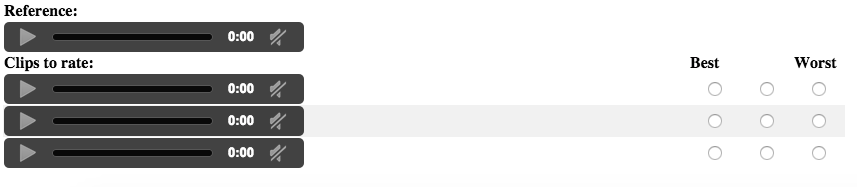
\includegraphics[scale=0.3]{mturk_task}
\caption{Question portion of an example Mechanical Turk task. Each task had two questions like these as well as a description of how to answer the questions.}
\end{figure}

\subsubsection{Results}
We took all of the rankings provided by workers and interpreted them as pairwise rankings. For example, if a worker rated systems $A$, $B$, and $C$ in that order, then that would be interpreted as $A>B, A>C,$ and $B>C$. Since ties were allowed, it could also look like $A>B, A>C$ and $B=C$. 

Figure 5 shows the results of the Mechanical Turk tasks. Specifically, it gives the percentage of workers that voted the latest model of MelTS with optimized weights as better, equal to, and worse than the other three systems (as compared to the Bach reference). The latest version of MelTS was rated better than U-AMP on approximately 55\% of tasks that compared the two, the largest difference in votes by a large margin. It was rated as equal in about 23\% of these tasks, and worse by the remaining 22\%. In fact, even the other two iterations of MelTS, one with unweighted features and the other with no phrase based model, were both rated better than U-AMP by a significant amount.

In addition, the different iterations of MelTS were evaluated to be an increase in quality over the last, although not by as wide of a margin as the one between U-AMP and the final iteration of MelTS. As is shown in Figure 5, the current version of MelTS was rated as better than the previous versions more often than it was rated worse or equal. The second iteration of MelTS was also rated better than the first iteration more often than it was rated equal or worse. Therefore, all successive iterations of MelTS were justified by human evaluation.

\begin{figure}
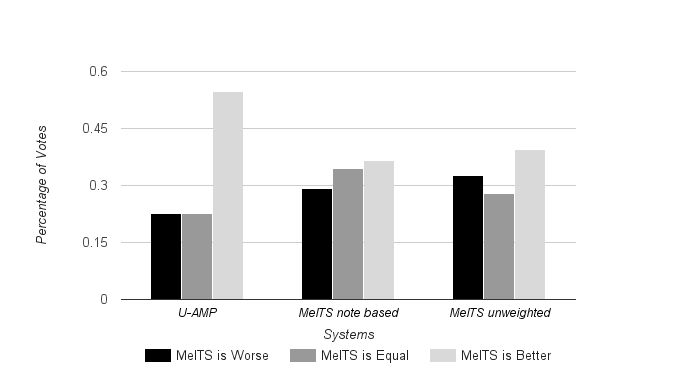
\includegraphics[scale=0.4]{mturk_results}
\caption{Results of Mechincal Turk Tasks - last iteration of MelTS versus all other systems.}
\end{figure}
\label{sec:system_performance}

\section{Ethics}
As with most artificial intelligence applications, an obvious ethical concern with this system is its potential impact on people whose activities it attempts to mimic. If MelTS produced compositions with such high quality that they were competitive with the compositions of modern professional composers, the system may threaten the livelihoods of composers and musicians. However, the authors believe that such a high level of output quality is so far in the future that this hypothetical situation could not be considered a legitimate concern.

If MelTS were to be widely used as an aid to musicians, there would be some foreseeable legal issues regarding ownership of the compositions. For example, would the composers of the training data have a right to the output? Would the output belong to the composer of the input harmony? To the creators of MelTS? Since music is generally considered intellectual property, it is clear that ownership of the output would need to be delineated to all users and composers of training data, but what the delineation might be is not immediately obvious.
\label{sec:ethics}

\section{Remaining Work}
A natural next step for MelTS would be to release the system to the public, preferably as a web application that would allow users to generate harmonies based on pre-computed models. Musicians could use the tool to experiment with harmonization ideas by exploring the way different genres of music would harmonize their melodies. Additionally, feedback from real users of the application would allow for further improvements to the system. 

In order to publish a viable a web app, the generation algorithm would need to be optimized for time efficiency. Minimal work has been done to systematically identify bottlenecks in the algorithm, although parallelization appears to be a clear way of speeding up. For example, generating all remaining parts based on the previously generated parts and extending harmony hypotheses during decoding can all be done in parallel.

Another future goal is to train more models in different styles of music. Potential styles would be marching band arrangements, orchestral scores, and gospel music. With some creativity in building the models, MelTS could even be used to generate chord accompaniment for pop songs.

As for improvements to the system itself, it would be interesting to investigate adding more features to the weighted log-linear score. For example, the chords for a beat could be predicted and incorporated into the score through a feature that captures whether or not the harmonized notes occur in one of the top predicted chords. To maintain a legal range of pitches within parts, a feature representing a note's distance from the center of the pitch range for a given part could also be incorporated.
\label{sec:remaining_work}


\bibliographystyle{plain}     % Please do not change the bib-style
\bibliography{progress_report}  % Just the *.BIB filename

\label{app}


\end{document} 

